\chapter{Annexes}


\section{Configuration prérequise pour l'utilisation des outils }

Avant d'utiliser le logiciel, l'utilisateur doit tout d'abord s'assurer d'avoir un environnement Java, ou \textbf{JRE} sur sa machine. Les explications nécessaires peuvent être trouvées sur le site suivant: \url{http://www.siteduzero.com} \\

L'utilisateur doit également disposer d'un accès à une base de données spatiale PostGIS. Pour ceci, il y a deux possibilités: L'utilisateur installe ou a déjà installé PostgreSQL et PostGIS en local sur sa machine (en local). Sinon, il existe également la possibilité de se connecter à une base de données stockée en ligne. Afin de pouvoir traiter et gérer des données raster, il faut que la version 2.0 de PostGIS soit installée. La possibilité de se connecter à une base de données distante augmente les possibilités de réutilisation du logiciel.\\

Finalement, l'utilisateur doit également avoir installé sur sa machine le logiciel R, ainsi les "packages" suivant: \\
\begin{itemize}
\item rgdal
\item RPostgreSQL
\item raster
\item spatstat
\item maptools
\end{itemize}

A l'instant, toutes les fonctionnalités peuvent être utilisées sous Linux et sous MacOS. Sous Windows, un certain nombre de fonctionnalités ne sont pas disponibles (cf Difficultés rencontrées).

\section{Packages R utilisés}



\textit{rgdal\\}

Rgdal est une extension de R et permet d'utiliser les fonctionnalités de la bibliothèque GDAL à partir du langage de programmation R. Cette extension permet donc tout d'abord de gérer et de représenter des fichiers spatiaux, mais également d'effectuer des traitements statistiques sur les objets géographiques.\\

\textit{RPostgreSQL\\}

RPostgreSQL fournit une interface de gestion permettant d'accéder aux bases de données PostgreSQL et au driver PostgreSQL pour R. Cet outil est particulièrement intéressant car il permet de se connecter à la base de données spatiale de la chaîne de traitements et d'y récupérer les données nécessaires pour les traitements sous R.\\

\textit{spatstat\\}

Spatstat est un libraire de R permettant de traiter et d'analyser des données spatiales. Ainsi, il permet par exemple de calculer une densité des points.\\

\textit{raster\\}

Raster est un paquet de R permettant de traiter les images raster. Ce paquet permet également de créer des fichiers raster à partir de données d'entrée de formats diverses.\\

\textit{maptools\\}

Paquet permettant de lire et de traiter des données géographiques comme par exemple des données au format shape (".shp").


\newpage


\section{Les traitements effectués par la chaîne de traitements fermée}

Pour chaque traitement effectué, la chaîne utilise différentes librairies et outils. Dans cette partie du travail, chaque traitement est expliqué en détail et quelles opérations informatiques ont été utilisées pour effectuer les différents traitements. Les traitements sont divisés en trois catégories (cf. Catégories des traitments):\\ 
\begin{itemize}
\item pré-traitements 
\item traitements 
\item post-traitements

\end{itemize}. 


\subsubsection{Pré-traitements}

\subsubsection{Modification du système de coordonnées}
L'utilisateur peut choisir individuellement les données d'entrée (ici les fichiers de forme Végétation, Bâtiments et Eau) en fonction de ses besoins. Il est donc nécessaire d'homogénéiser les systèmes de coordonnées de ces données. Ceci est fait lors de la transformation des fichiers vecteurs (shape), à l'aide de la commande shp2pgsql. \\

\textbf{Librairies utilisées:} PostgresSQL, PostGIS, JDBC 

\textbf{Données en entrée:} Fichiers de forme géoréférencés (vecteur)

\textbf{Données temporaires:} Fichiers .sql

\textbf{Données en sortie:} Données avec système de coordonnées dans base de données\\


\begin{algorithm}[H]
\caption{\label{traitement1} shp2pgsql}
Syntaxe:
shp2pgsql -d -g nomGeom -s SRID fichier.shp nomTable -> fichier.sql \\
%Exemple: 
%shp2pgsql -d -g geom\_batiments -s 32360 batiments.shp batiments -> batiments.sql
\end{algorithm}

Pour la modification de la projection, c'est l'option -s SRID de la commande "shp2pgsql" qui va effectuer cette opération. Cette option définit le système de coordonnées ou, s'il existe déjà, le modifie. A l'intérieur de la chaîne de traitements, cette option est définie une seule fois  lors de la création de la base de données et toutes les données vectorielles insérées dans la base de données auront le même système de coordonnées afin de garantir l'homogénéité de l'ensemble des données.




\subsubsection{Création base de données}

Il existe plusieurs moyens pour créer une base de données. Nous utilisons la méthode suivante: Connexion à la base de données de maintenance "postgres" et création d'une nouvelle base de donnée. Attention, cette base de données n'est pas encore compatible avec les données spatiales (géographiques).\\

\textbf{Librairies utilisées:} PostgresSQL, PostGIS, JDBC 

\textbf{Données en entrée:}  /

\textbf{Données en sortie:} Base de données PostgreSQL \\

\begin{algorithm}[H]
\caption{\label{traitement3} create database}
Syntaxe:
CREATE DATABASE nomBase\\
\end{algorithm}

\subsubsection{Initialisation de la base de données aux fonctionnalités PostGIS}

Il est nécessaire d'inclure 3 fichiers dans la base de données afin de la rendre compatible avec les fonctionnalités PostGIS: postgis.sql, spatial\_ref\_sys.sql, rtpostgis.sql.\\

\begin{itemize}
\item postgis.sql: Permet de charger dans la base de données, les types, les fonctions géographiques et les tables associées qui sont utilisées avec PostGis.
\item spatial\_ref\_sys.sql: Permet de charger dans la base de données, la table spatial\_ref\_sys qui contient environ 300 systèmes de référence spatiales et les détails nécessaires à leur transformation.
\item rtpostgis.sql: Permet de charger dans la base de données les fonctionnalités nécessaire pour qu'elle supporte les fichiers raster.\\
\end{itemize}

\textbf{Librairies utilisées:} PostgresSQL, PostGIS, JDBC 

\textbf{Données en entrée:} Base de données PostgreSQL

\textbf{Données en sortie:} Base de données PostgreSQL compatible PostGIS \\

\begin{algorithm}[H]
\caption{\label{traitement4} Initialisation base de données PostGIS}
Syntaxe:
psql -d nomBase -f postgis.sql (pareil pour spatial\_ref\_sys.sql et rtpostgis.sql)\\
\end{algorithm}

\subsubsection{Traitements}

\subsubsection{Transformation du format de fichier}

Afin de pouvoir insérer des fichiers de forme vecteur dans une base de données spatiale il est nécessaire de les transformer. Cette transformation est également effectuée à l'aide du module de transformation shp2pgsql intégré dans PostGIS. L'option -d de cette fonction indique au module de supprimer la table si elle existe déjà dans le base de données et de la recréer par la suite. Cette option permet donc de garantir que les données en entrée seront insérées correctement dans la base de données. L'option -g permet de choisir le nom de la colonne géométrique (créée automatiquement pour toute couche géométrique insérée dans une base de données PostgreSQL / PostGIS) ce qui facilitera les traitements par la suite. L'option -s a été détaillée ci-dessus et permet de choisir le système de coordonnées de la donnée. L'option "nomtable" attribue le nom de la table dans la base de données correspondant à la donnée d'entrée. Le paramètre "fichier.sql" indique l'emplacement du fichier ".sql" en sortie qui sera par la suite utilisé pour insérer les données dans la base de données.\\

\textbf{Librairies utilisées:} PostgresSQL, PostGIS, JDBC 

\textbf{Données en entrée:} fichiers de forme géoréférencés (vecteur)

\textbf{Données en sortie:} Fichiers au format .sql \\

\begin{algorithm}[H]
\caption{\label{traitement2} shp2pgsql}
Syntaxe:
shp2pgsql -d -g nomGeom -s SRID fichier.shp nomTable -> fichier.sql \\
%Exemple: 
%shp2pgsql -d -g geom\_batiments -s 32360 batiments.shp batiments -> batiments.sql
\end{algorithm}

La fonctionnalité "ogr2ogr" de la bibliothèque GDAL  peut également être utilisée, notamment pour des conversions vers d'autres formats  que le format ".sql".

\subsubsection{Calcul de la surface totale d'une couche de données}

La surface totale d'une couche de données est calculée à l'aide de la fonction PostGIS suivante: ST\_AREA(geom\_couche). Cette fonction calcule la surface totale pour chaque enregistrement d'une colonne géométrique d'une table. L'unité correspond automatiquement à l'unité du système de coordonnées de la base de données. A partir de ce calcul on obtient facilement la surface totale à l'aide d'une requête SQL classique (select SUM...).\\

\begin{algorithm}[H]
\caption{\label{traitementstat1} Calcul surface}
Syntaxe:
SELECT ST\_AREA(geom\_table) from table as somme\\
\end{algorithm}

\subsubsection{Calcul densité de population et taille pixel} 

Dans les zones de risque, les habitations sont généralement des habitations sur un seul étage. Ainsi, il est possible de calculer à partir de la surface totale des bâtiments et de la population totale de la ville, la superficie qu'occupe en théorie un seul habitant. \\
Par exemple, pour une population de 15.000 habitants sur une superficie totale de 300.000 m2, nous effectuons le calcul suivant: \\

300.000/15.000 = 20 m2 par habitants.\\

Un habitant correspond donc en théorie à 20 mètres carrés. A partir de ce calcul, nous pouvons déterminer la taille théorique d'un pixel. Pour les données d'essai utilisées, ce sont donc les calculs suivants qui sont effectués lors du lancement de la chaîne de traitements: \\
 
14 133 habitants =  249394,70358 mètres carrés  

1 habitant = 17,646 mètres carrés

1 pixel = 4.2 m * 4.2 m\\

Aucune fonctionnalité particulière n'est nécessaire pour ce calcul statistique, Java ou R peuvent facilement effectuer ces calculs de base.


\subsubsection{Insertion fichiers de forme dans une base de données spatiale}

Pour l'insertion d'un fichier de forme dans une base de données les informations suivantes sont nécessaires: le serveur (en général localhost), le port sur lequel la base de données est installé (en général 5432), le nom de l'utilisateur qui est le propriétaire de la base de données, le nom de la base de données dans laquelle seront insérées les fichiers de forme et enfin le fichier ".sql" qui comporte les informations relatives au fichier de forme transformé par avant.\\

\textbf{Librairies utilisées:} PostgresSQL, PostGIS, JDBC 

\textbf{Données en entrée:}  Fichiers au format .sql(vecteur)

\textbf{Données en sortie:} Table dans la SGBD \\

\begin{algorithm}[H]
\caption{\label{traitement5} psql}
Syntaxe:
psql -h serveur - p port -U Utilisateur -d nomBase -f fichier.sql\\
\end{algorithm}

\subsubsection{Buffer}

Afin de pouvoir déterminer et représenter l'aléa lié au risque, il est nécessaire de créer des buffers (zones tampons) autour des points d'eau. Ce traitement est effectué à l'aide de la fonctionnalité Postgis "ST\_Buffer". Les informations obtenues sont stockées dans une nouvelle table à l'intérieur de la base de données, ce qui permet en même temps de créer une nouvelle table de données dans la base de données. A noter qu'il faut utiliser la colonne géométrique de la couche par rapport à laquelle on veut calculer les buffers.\\

\textbf{Librairies utilisées:} PostgresSQL, PostGIS, JDBC 

\textbf{Données en entrée:}  Table géométrique dans une BDS

\textbf{Données en sortie:}  Table géométrique dans une BDS \\


\begin{algorithm}[H]
\caption{\label{traitementbuffer} Buffer 400 mètres}
Syntaxe pour un buffer de 400 mètres autour de la couche eau:
create table buffer\_eaux400 as select gid, st\_buffer(geom\_eaux,400) from eaux;\\
\end{algorithm}

Cette opération crée des zones tampons autour de chaque point d'eau de la couche de source et donc plusieurs géométries différentes.

\subsubsection{Union}

La création de buffers crée plusieurs géométries différentes à l'intérieur d'une table. Pour la suite des traitements il est nécessaire de créer une seule géométrie à partir des différentes géométries. Il faut donc disposer d'une géométrie unique pour la table buffer\_eaux400 par exemple. Cette opération est effectuée à l'aide de la fonctionnalité "ST\_UNION" de Postgis. Le résultat de cette opération est stocké dans une nouvelle table de la base de données. \\

\textbf{Librairies utilisées:} PostgresSQL, PostGIS, JDBC 

\textbf{Données en entrée:}  Table géométrique dans une BDS

\textbf{Données en sortie:}  Table géométrique dans une BDS \\

\begin{algorithm}[H]
\caption{\label{traitementunion} Union de plusieurs géométries}
Syntaxe:
create table tableNom as select st\_union(st\_geom) from table;\\
\end{algorithm}


\subsubsection{Intersection}

La création de zones tampons crée logiquement des géométries se situant à l'extérieur de notre zone d'étude. Pour enlever cette partie d'information, qui va seulement ralentir le déroulement de notre chaîne de traitements, nous l'enlevons en utilisant la fonctionnalité Postgis "ST\_INTERSECTION". Nous créons une intersection des géométries des buffers par rapport à "l'emprise" de notre zone d'étude. 
\\


\textbf{Librairies utilisées:} PostgresSQL, PostGIS, JDBC 

\textbf{Données en entrée:}  Table géométrique dans une BDS

\textbf{Données en sortie:}  Table géométrique dans une BDS \\

\begin{algorithm}[H]
\caption{\label{traitementintersect} Intersection de plusieurs géométries}
Syntaxe:
create table raster4001 as select st\_intersection(st\_geom,st\_envelope) from table1,extend;\\
\end{algorithm}


\subsubsection{Différence entre deux couches géométriques}

Il peut être nécessaire de calculer la différence entre deux géométries. La fonctionnalité à utiliser dans ce cas est la fonctionnalité Postgis "ST\_SymDifference". \\

\textbf{Librairies utilisées:} PostgresSQL, PostGIS, JDBC 

\textbf{Données en entrée:}  Table géométrique dans une BDS

\textbf{Données en sortie:}  Table géométrique dans une BDS \\

\begin{algorithm}[H]
\caption{\label{traitementsymdiff} Différence entre deux géométries}
Syntaxe:
select ST\_SymDifference(a.st\_geom,b.st\_geom) from table1 a, table2 b\\
\end{algorithm}



\subsubsection{Rastérisation d'un fichier de forme}

Afin de traiter la couche "batiments" il est nécessaire de la transformer en raster. Ceci est fait en utilisant la commande PostGIS "select ST\_ASRaster" qui transforme la colonne géométrique d'une table en colonne de type "raster". Au stade de développement actuel de Postgis, il est indispensable que la nouvelle colonne s'appelle "rast", sinon les autres fonctionnalités (rgdal par exemple) n'arrivent pas à lire et à traiter l'information. La taille du pixel calculée par avant est également réutilisée et chaque pixel du raster aura la taille calculée par avant.\\

\textbf{Librairies utilisées:} PostgresSQL, PostGIS, JDBC 

\textbf{Données en entrée:}  Fichiers au format .sql(vecteur)

\textbf{Données en sortie:} Table "raster" dans la SGBD \\

\begin{algorithm}[H]
\caption{\label{traitement6} Transformation table batiments en table raster}
Syntaxe:
CREATE TABLE bati\_raster as SELECT ST\_asraster(geom\_batiments,taillePixel,-taillePixel)  as rast from batiments")\\
\end{algorithm}

Cette opération peut également être effectuée sous R à l'aide de la librairie "raster" et de la fonction "rasterize". Les tests ont néanmoins démontré que Postgis est beaucoup plus rapide pour faire ce genre de traitement.

\subsubsection{Emprise d'une couche}

Afin de délimiter d'autres données et informations par rapport à notre zone d'étude, il est nécessaire de connaître l'étendu de la zone. La fonctionnalité Postgis "ST\_ENVELOPE" effectue cette opération. En sortie, nous obtenons une géométrie qui représente (sous forme de rectangle) l'emprise d'une couche. Par la suite nous pouvons intersecter les autres données par rapport à cette géométrie. (cf \ref{traitementintersect} )\\

\textbf{Librairies utilisées:} PostgresSQL, PostGIS, JDBC 

\textbf{Données en entrée:}  Table dans une BDS(vecteur)

\textbf{Données en sortie:} Table dans une BDS \\

\begin{algorithm}[H]
\caption{\label{traitementemprise} transformation table géométrique en table raster}
Syntaxe:
create table extend as SELECT st\_envelope(rast) from densite\_batiment \\
\end{algorithm}

\subsubsection{Chargement d'une donnée raster dans R à partir d'une base de données spatiale}

Pour charger une donnée raster stockée dans une base de données spatiale nous utilisons la fonctionnalité "readGDAL" de la librairie "rgdal" du logiciel R. \\

\textbf{Librairies utilisées:} PostgresSQL, PostGIS, R, rgdal, RPostgreSQL 

\textbf{Données en entrée:} Table dans une BDS(vecteur)

\textbf{Données en sortie:} Variable R (raster)\\

\begin{algorithm}[H]
\caption{\label{chargerraster} Charger données raster dans R à partir d'une base de données spatiale}
Syntaxe:
layers <- readGDAL("PG:host="hote" user="username" dbname="nomBase" password="mot de passe" port="port" table=coucheRaster" \\
\end{algorithm}

La même opération peut être effectuée avec des données au format vectoriel et la fonctionnalité "readOGR" de la même librairie R.\\
Illustration de la couche "batiments" chargée à partir de la base de données PostgreSQL / Postgis:

\begin{center}
\begin{figure}[h] \centering 
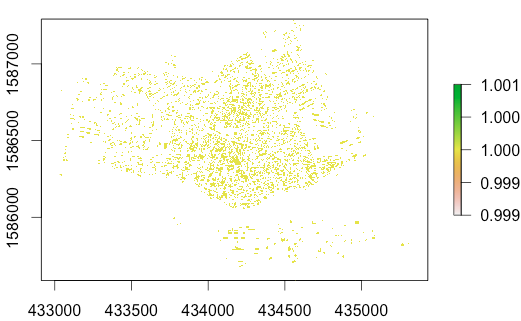
\includegraphics[width=10cm]{rasterbati2}\\
\caption{\label{rasterbati} Raster chargé dans R}
\end{figure}
\end{center}


\subsubsection{Transformation d'une couche raster en points}

Afin de représenter la densité de population, nous allons calculer une densité des points. Il est donc nécessaire de transformer le raster (pour lequel un pixel correspond aux calculs effectués par avant) en points. Chaque pixel correspondra donc à un point. Le logiciel R avec sa libraire "raster" permet d'effectuer ce genre d'opération grâce à la commande "rasterToPoints".\\

\textbf{Librairies utilisées:} R, RCaller, rgdal 

\textbf{Données en entrée:}  Table raster dans BDS

\textbf{Données en sortie:} Fichier de points dans R\\

\begin{algorithm}[H]
\caption{\label{traitementpoints} Transformation d'une couche raster en points}
Syntaxe:
rasterToPoints(raster,fun=function(x){x>0},spatial=TRUE) \\
\end{algorithm}

L'opération nécessite tout d'abord une variable R au format R (chargée depuis la base de donnée spatiale dans notre cas). Par la suite la fonction "fun=function(x){x>0}" permet de ne pas prendre en compte tous les pixel "vides". \\

Illustration de la couche "batiments" chargée à partir de la base de données PostgreSQL / Postgis

\begin{center}
\begin{figure}[h] \centering
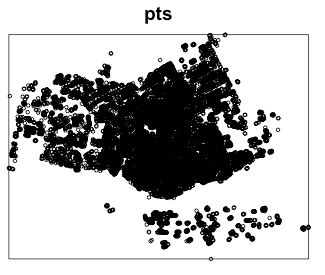
\includegraphics[width=10cm]{pointsbati2}\\
\caption{\label{poitsbati} Raster transformé en points}
\end{figure}
\end{center}

\subsubsection{Calcul densité des points}

Pour calculer la densité des points, nous utilisons la librairie "spatstat" de R. 2 opérations différentes sont nécessaires: D'abord il faut transformer la variable au format points vers le format compatible spatstat qui est "ppp (point pattern)". Par la suite on peut calculer la densité à partir de cette variable à l'aide de la commande "density.ppp".\\

\textbf{Librairies utilisées:} R, spatstat

\textbf{Données en entrée:}  Variable R (points)

\textbf{Données en sortie:} Variable R (points pattern, densité des points)\\

\begin{algorithm}[H]
\caption{\label{traitementdesite} Densité des points}
Syntaxe:
pts <- as(points,ppp)\\
dsty <- density.ppp(pts,eps=taillePixel,taillePixel ,adjust=taillePixel)\\
\end{algorithm}

L'argument "eps" permet de définir la taille des pixels de la variable en sortie. Si on n'ajoute pas cet argument, R calcule automatiquement la taille des pixels en sortie. Il est donc important d'indiquer la taille de pixel calculée par avant pour obtenir le résultat souhaité. 
L'argument "adjust" permet à l'utilisateur de déterminer le "lissage du pixel en sortie". La fonctionnalité "density.ppp" offre un large nombre de possibilité pour régler ce paramètre. Plusieurs essais ont montré que le plus facile est d'utiliser l'argument "adjust" qui est une combinaison entre toutes les autres possibilités. Cet argument va par exemple multiplier le "sigma" automatiquement par cette valeur. A nouveau, il faut attribuer à cet argument comme valeur la taille du pixel calculée par avant.\\
Illustration des résultats selon les arguments utilisés:

\begin{center}
\begin{figure}[h] \centering
\includegraphics[width=16cm]{3Densites}\\
\caption{\label{3densites} Densités des points selon les paramètres}
\end{figure}
\end{center}

\subsubsection{Rastériser une couche de points}

Afin de pouvoir exporter une variable R représentant une densité de points (la variable R est au format "ppp") il est nécessaire tout d'abord de la transformer vers le format "SpatialGridDataFrame". Par la suite, il est facilement possible de transformer ce format en format raster à l'aide de la fonction "raster(...)".\\

\textbf{Librairies utilisées:} R, spatstat, raster

\textbf{Données en entrée:}  Variable R (densité de points)

\textbf{Données en sortie:} Variable R (raster)\\

\begin{algorithm}[H]
\caption{\label{traitementpointsverraster} Transforamtion points en raster}
Syntaxe:
ab <- as(densitePoints,"SpatialGridDataFrame")\\
ras <- raster(ab)
\end{algorithm}

\subsubsection{Reclassification d'une couche raster}

Chaque pixel du raster créé contient une valeur en fonction de la densité des points calculée par avant. Afin d'optimiser le résultat, il est nécessaire de faire une reclassification de l'image raster. Nous allons classifier l'image en 4 catégories: les pixels vides auront la valeur 0. Les autres pixels seront regroupés en 3 classes égales.\\

\textbf{Librairies utilisées:} R, raster

\textbf{Données en entrée:}  Variable R (raster)

\textbf{Données en sortie:} Variable R (raster reclassifié)\\

\begin{algorithm}[H]
\caption{\label{reclassification} Transformation points en raster}
Syntaxe:
maxim <- maxValue(ras)\\
minim <- minValue(ras)\\
somme <- maxim+minim\\
sixieme <-somme/6\\
tiers <-sixieme*2\\
m <- c(minim-1,0,0,0.0001, sixieme,1, sixieme,tiers,2, tiers,maxim,3)\\
rclmat <- matrix(m, ncol=3, byrow=TRUE)\\
rc <- reclass(ras,rclmat)\\
\end{algorithm}

Illustration des résultats avant et après la reclassification:

\begin{center}
\begin{figure}[h] \centering
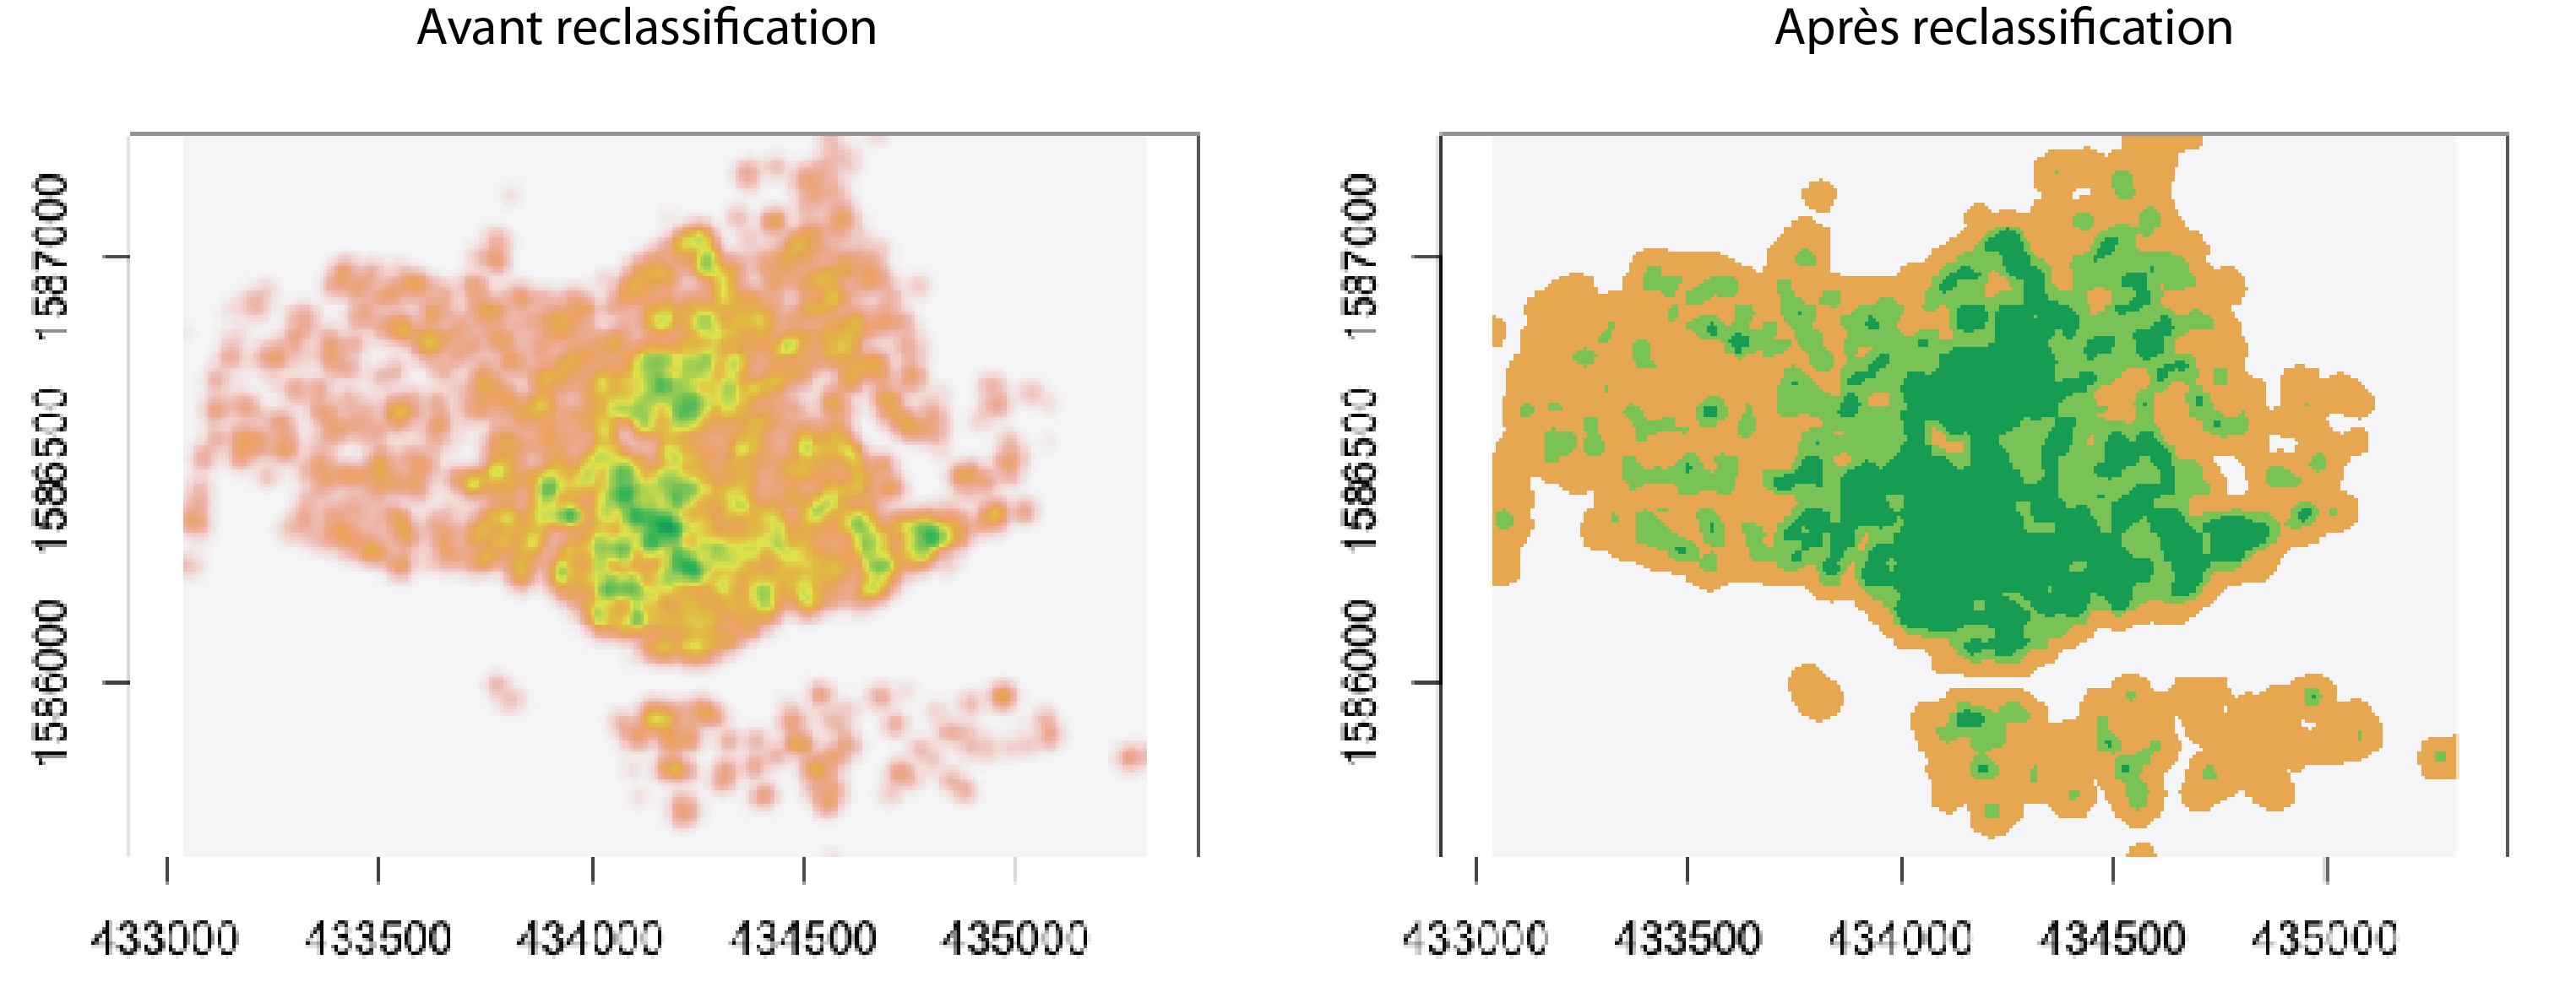
\includegraphics[width=14cm]{reclassification}\\
\caption{\label{reclassifications} Reclassification d'une image raster}
\end{figure}
\end{center}


\subsubsection{Post-traitements}

\subsubsection{Combinaison de plusieurs couches raster}

La combinaison de deux couches raster nous permet d'obtenir une combinaison entre la carte de vulnérabilité (=carte de densité des points) et la carte d'aléas (=carte buffers). La fonctionnalité à utiliser est "mosaic" de la librairie "raster".\\

\textbf{Librairies utilisées:} R, raster

\textbf{Données en entrée:}  2 données raster

\textbf{Données en sortie:} 1 donnée raster\\

\begin{algorithm}[H]
\caption{\label{mosaic} Combinaison de deux données raster}
Syntaxe:
mosaic(raster1,raster2,fun=sum)
\end{algorithm}

L'argument "fun" de cette fonction indique la méthode selon laquelle les deux raster sont combinés. Nous utilisons la méthode "sum" (somme) qui va donc calculer la somme des valeurs des pixels des raster combinés.


\section{Divers}

\subsection{Planning provisionnel}


\begin{center}
\begin{figure}[h] \centering
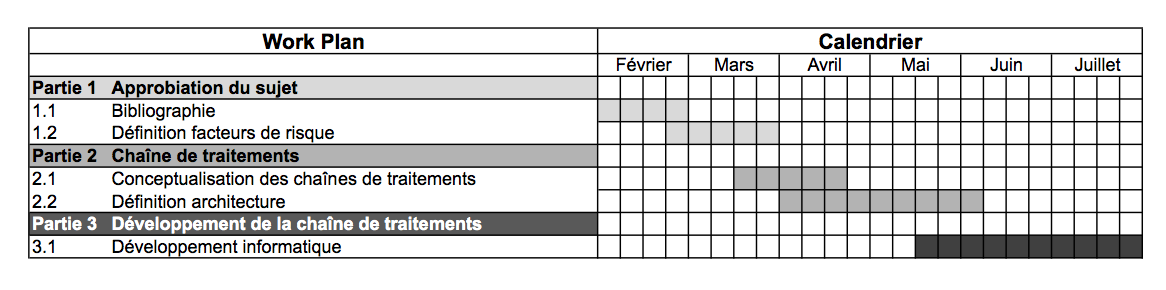
\includegraphics[width=14cm]{GanttProvisoire}\\
\caption{\label{GanttProvisoire} Planning provisionnel}
\end{figure}
\end{center}


